There are some practical challenges involved in implementing this approach in
practice, including:

\begin{outline}
\1 Need a way to fuzz traces and replay them: network simulator.

\1 Need visibility into as many internal events as possible: optional
interposition on logging

\1 Need to cope with non-determinism in the operating system: multiplexed sockets
and overriding gettimeofday()

\1 Can't squash all the non-determinism: replaying multiple times yields
Bernoulli probability that bug won't be triggered
\end{outline}

\subsection{Simulated Execution}
\label{subsec:simulation}

Unlike the example applications described
by the original delta debugging paper~\cite{Zeller:1999:YMP:318773.318946}, the system we are troubleshooting is not a
single program--it is all the nodes and links of a distributed system,
including controllers, switches, and end-hosts. The asynchrony of distributed
systems makes it difficult to reliably replay orderings of
events without great care. We therefore simulate the control-plane
behavior of network devices (with support for minimal data-plane behavior) on
a single machine. We then run the control software on
top of this simulator and connect the software switches to the controllers as if they were true
network devices, such that the controllers believe they are configuring a true
network. This setup allows the simulator to interpose on all communication
channels. The simulator uses these interposition points to delay, drop, or reorder
messages as needed for replay. The overall
simulation architecture is depicted in
Figure~\ref{fig:architecture}.

\begin{figure}[t]
    %\hspace{-10pt}
    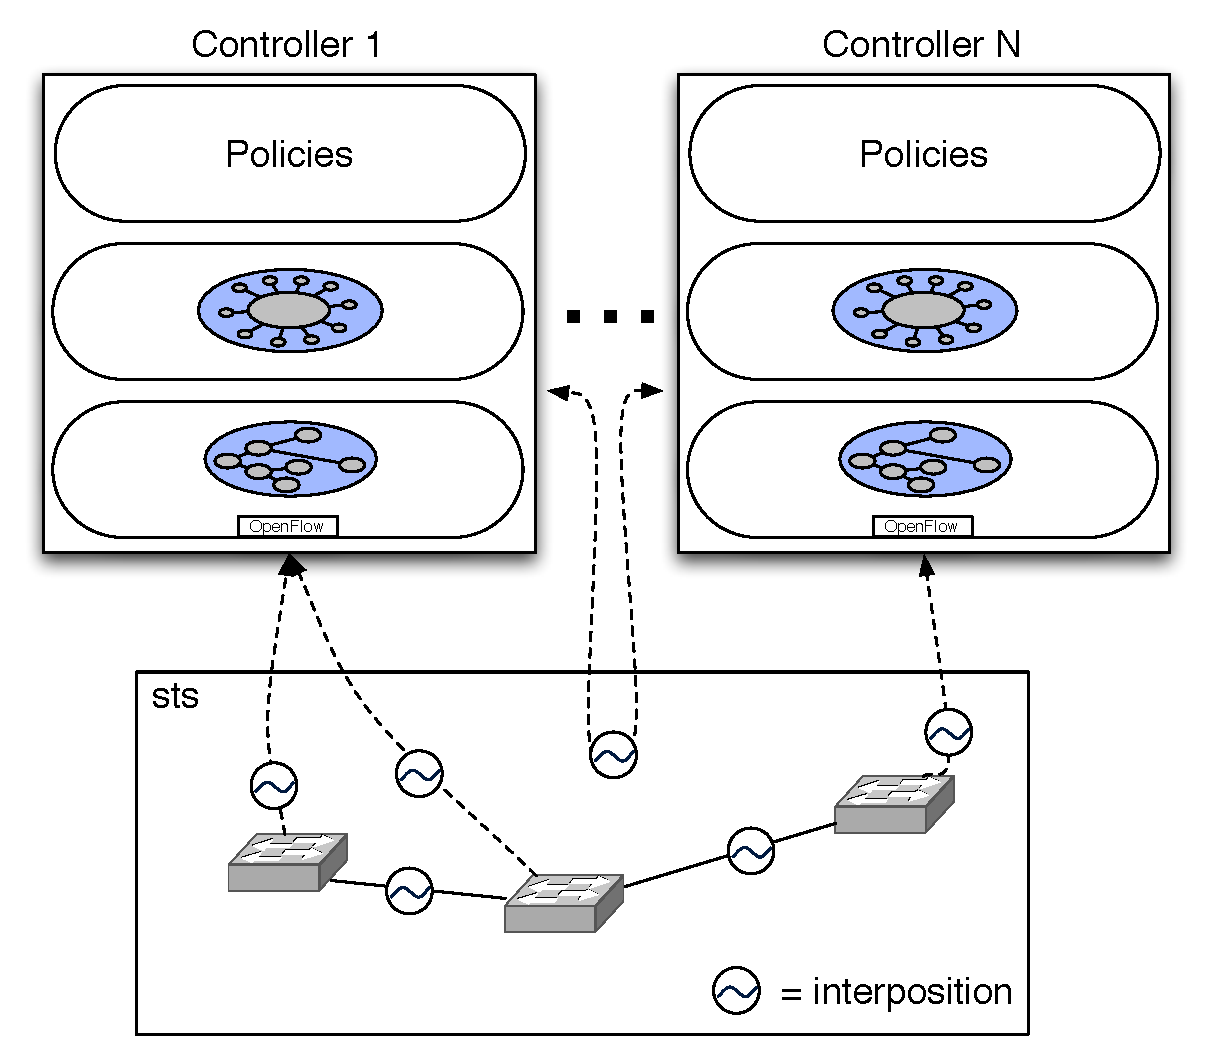
\includegraphics[width=3.25in]{../diagrams/architecture/Debugger_Architecture.pdf}
    \caption[]{\label{fig:architecture} Simulation infrastructure. We simulate
    network devices in software, and interpose on all communication
    channels.}
\end{figure}

Given a sequence of inputs (\eg~link failures, controller crashes, host migrations,
or policy changes) and an invariant checking probe (provided by tools
such as HSA~\cite{hsa,hsa_realtime} or Anteater~\cite{anteater,khurshid2012veriflow}),
delta debugging finds a minimal causal sequence responsible for triggering the
policy violation. The
simulator is responsible for replaying intermediate input subsequences
chosen by delta debugging. For example, the simulator replays link failures
by disconnecting the edge in the simulated network, and sending a
port status message from the adjacent switches to their parent controller(s).

The input subsequences chosen by delta debugging are not always valid. For
example, it is not sensible to replay a recovery event without a
preceding failure event; nor is it sensible to replay a host migration
event without modifying its starting position when a preceding host
migration event has been pruned. The simulator checks
validity before replaying a given subsequence to account for this
possibility.\footnote{Handling invalid inputs is crucial for
ensuring that the delta debugging algorithm we employ~\cite{Zeller:1999:YMP:318773.318946}
is guaranteed to find a minimal causal sequence, since it assumes that no unresolved
test outcomes occur. Zeller wrote a follow-on
paper~\cite{Zeller:2002:SIF:506201.506206} that removes the need for this assumption,
but incurs an additional factor of $N$ in complexity in doing so.}
Currently our simulator accounts for validity of all network state change
events (shown in Table \ref{tab:inputs}), but does not support policy changes,
which have more complex semantics.

